\section*{Neural Networks}

$F(x)=W^{L}\phi^{L-1}(W^{L-1}...(\phi^{1}(W^{1}x)...))$

$\textbf{ReLU: } \max (0,z), \; \textbf{Tanh: } \frac{\exp(z) - \exp(-z)}{\exp(z) + \exp(-z)}$ \\[-3pt]
$\textbf{Sigmoid: } \varphi(z) = \frac{1}{1 + \exp(-z)}, \varphi' = (1 - \varphi) \varphi$

\begin{rowlist}
    \item vanishing G.: sigm, tanh
    \item non-linear: I, ReLu for $\geq 0$ \& sigm around 0
    \item diff: all but ReLU at 0
    \item $\mu = 0$ : I, others shift to $\uparrow \mu$
    \item ReLU edgy \& tanh, sigm smooth b.

\end{rowlist}


\textbf{Universal Approximation Theorem}: We can approximate any arbitrary smooth target function, with 1+ layer with sufficient width.

\subsection*{Forward Propagation}

Input: $v^{(0)} = [x; 1]$ \quad Output: $f = W^{(L)} v^{(L-1)}$
Hidden: $z^{(l)} = W^{(l)} v^{(l-1)}, v^{(l)} = [\varphi(z^{(l)}); 1]$


\subsection*{Backpropagation}

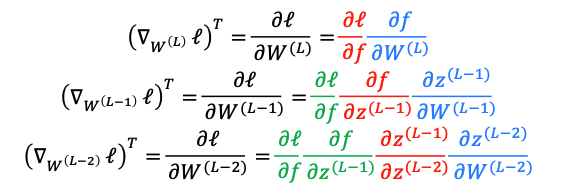
\includegraphics[width=\columnwidth]{backpropagation.png} \\[-15pt]

Weight initalization $\varphi \sim \mathcal{N}(0, \sigma)$ : $\sigma_{ReLU}=2 / n_{in}$, $\sigma_{tanh}=  1/n_{in} \text{ or } 1/ (n_{in} + n_{out})$)

\subsection*{Overfitting}
\textbf{Weight Decay} regularizes l2-norm; \textbf{Early Stopping}; \textbf{Dropout}: ignore hidden units with prob. $p$, after training use all units and scale weights by $p$; \textbf{Batch Normalization}: standardize the input in each layer

\subsection*{MLP \quad \color{Black}$\varphi(W \cdot v^{(l)}) + b$ \normalfont \textit{(fully c., ff-nn)} }
$\textbf{\#P}_{fc} = \sum_{m=1}^{L_{\text{fc}}} \left( (n_{\text{in}}^{(m)} \times n_{\text{out}}^{(m)}) + n_{\text{out}}^{(m)} \right)$


\subsection*{CNN \quad \color{Black}$\varphi(W * v^{(l)}) + b$ \normalfont \textit{(share weights, ff-nn)} }
$\textbf{\#P}_{conv} = \sum_{l=1}^{L_{\text{conv}}} \left( (k_h^{(l)} \times k_w^{(l)} \times c_{\text{in}}^{(l)} + 1) \times n_{\text{filters}}^{(l)} \right)
$
where $c_{\text{in}}^{(l)}$ =  $n_{\text{filters}}^{(l-1)}$ \& $\text{\#P}_{tot} = \text{\#P}_{conv} + \text{\#P}_{fc}$
$out_d = \frac{n_d + 2p - f_d}{s} + 1$  (ind. of \#channels)

n is input size \& f filter size of resp. d
